% \documentclass[aspectratio=169]{beamer} % includes \pause in render
\documentclass[aspectratio=169,handout]{beamer} % do not include \pause in render

\usetheme[neutralbackground]{uniamntf}

\title[Computer aided calculations]{\vspace{-2em}Computer aided Analytical Calculations for Physical Many-Body Problems}
\subtitle{ - Project Work Presentation - }

\author{Jonas Kell}
\institute[TP III]{Chair for theoretical Physics III}

\date[01.05.2024]{$15^{\text{th}}$ of Mai 2024}

\acknowledgement{
    Jonas Kell\\
    Augsburg University\\
    jonas.kell@student.uni-augsburg.de\\
    www.uni-augsburg.de
}

\newcommand{\blankfootnote}[1]{%
\let\thefootnote\relax\footnotetext{#1}%
}
\newcommand{\tab}{%
\,\,\,\,
}

% bibtex/biber
\usepackage[backend=biber, style=phys, biblabel=brackets]{biblatex} % citations with "modern" backend and an physics-accepted citation style
\addbibresource{literature.bib}

\newenvironment{wideitemize}{\itemize\addtolength{\itemsep}{0.3em}}{\enditemize}

\begin{document}

    \begin{frame}[t,plain] 
        \maketitle
    \end{frame}

    \begin{frame}
        \frametitle{Outline}
        \tableofcontents
    \end{frame}

    
\section{Introduction of the problem}
    
    \begin{frame}{Physics of what we calculate}
    \end{frame}

    \begin{frame}{Working on paper: A Computer-Scientists view}
    \end{frame}

\section{Solutions: Off the shelf}
    \begin{frame}
        \frametitle{title}
    \end{frame}

\section{Math-Manipulator}
    \begin{frame}
        \frametitle{title}
    \end{frame}

\subsection{What did I do?}
    \begin{frame}
        \frametitle{title}
    \end{frame}

\subsection{How can you use it}
    \begin{frame}
        \frametitle{title}
    \end{frame}

\section{Custom Python Scripts (Sympy)}
    \begin{frame}
        \frametitle{title}
    \end{frame}

    \section{Presentations? - Custom Beamer Template}
        \begin{frame}{Beamer: LaTeX way of writing Presentations}
            \begin{itemize}
                \item Write presentations like your papers/thesis    \pause
                \item Reuse formulas/images/code/sources    \pause
                \item Consistent style \& references    \pause
                \item Version control    \pause
                \item Easier collaboration
            \end{itemize}

            \blankfootnote{Beamer \cite{beamerPackageCtan} \tab{} Template \cite{selfBeamerTemplateMNTF}}
        \end{frame}

        \begin{frame}{Minimal example for beamer presentation}
            \begin{columns}
                \column{0.4\textwidth}
                    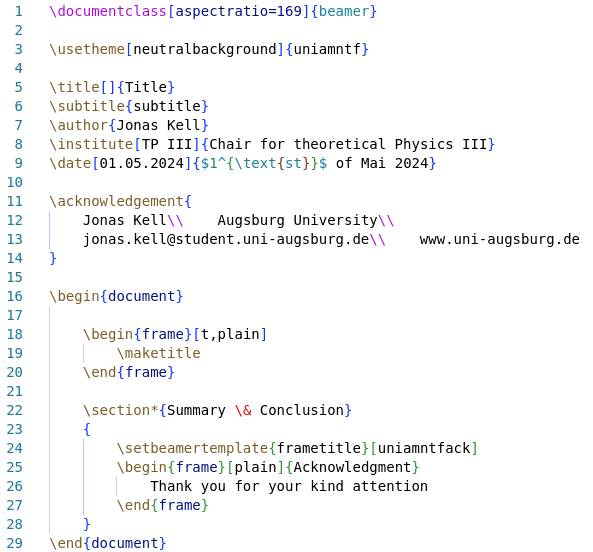
\includegraphics[width=1.1\textwidth]{./beamer-minimal-example/code.png}
                \column{0.4\textwidth}
                    
\includegraphics[width=0.9\textwidth]{./beamer-minimal-example/result.png}
            \end{columns}
        \end{frame}


    \section*{Summary \& Conclusion}
    {
        \setbeamertemplate{frametitle}[uniamntfack] % use the acknowledgment-style for this slide
        \begin{frame}[plain]{Acknowledgment}
            Thank you for your kind attention
        \end{frame}
    }
    \begingroup

    \begin{frame}[allowframebreaks,noframenumbering]
        \frametitle{References}
        \nocite{*}
        \printbibliography[title={Bibliography}]
    \end{frame}
    
    \section*{Extra slides}
        \begin{frame}[noframenumbering]{Theme alternative: Faculty of App. Computer Science}
            \hspace{1cm}\includegraphics[height=.7\paperheight]{./../latex-beamer-template/rendered-preview-pictures/FAICompilation.png}
        \end{frame}

\end{document}
